\chapter{System detekcji zachowań w czasie rzeczywistym}\label{cha:detektor}

Komponent detekcji zachowań stanowi główną warstwę analityczną wytworzonego systemu monitoringu wizyjnego. Jest to aplikacja działająca w trybie usługi mikroserwisowej wewnątrz izolowanego kontenera \texttt{Docker}, napisana w języku Python. Zadaniem modułu jest ciągła akwizycja strumieni wideo, wielopoziomowa analiza klatek obrazu pod kątem występowania specyficznych klas obiektów oraz dynamiki ludzkiego szkieletu, a także podejmowanie zautomatyzowanych decyzji o inicjacji zapisu weryfikowanego materiału na podstawie elastycznych szablonów reguł.



\section{Wykorzystane modele uczenia maszynowego}\label{sec:detektor_modele}

Rozwiązanie postawionego problemu badawczego wymagało połączenia modeli o różnej specyfice operacyjnej: klasycznej detekcji bounding-box, regresji punktów kluczowych oraz klasyfikacji szeregów czasowych. Wybór architektur podyktowany był koniecznością zachowania ścisłego kompromisu pomiędzy precyzją (\texttt{mAP}) a opóźnieniem inferencji na pojedynczej klatce.

\subsection{Detekcja obiektów: YOLOv26-m}
Do zadań ogólnej detekcji przedmiotów oraz lokalizacji pojazdów wyznaczono model \texttt{YOLOv26-m}. Architektury z tej rodziny charakteryzują się jednoprzebiegowym wyznaczaniem obwiedni oraz wysoką odpornością na rozmycie w ruchu. Bazowy model docelowo operuje na 9 zdefiniowanych klasach istotnych z punktu widzenia bezpieczeństwa publicznego: człowiek (\texttt{human}), rower (\texttt{bicycle}), samochód (\texttt{car}), ptak (\texttt{bird}), kot (\texttt{cat}), pies (\texttt{dog}), plecak (\texttt{backpack}), walizka (\texttt{suitcase}) oraz nóż (\texttt{knife}). 

Każdemu wykrytemu obiektowi przypisywany jest unikalny identyfikator instancji śledzony pomiędzy kolejnymi klatkami za pomocą algorytmu asocjacji przestrzennej. Pozwala to wyeliminować problem wielokrotnego zliczania tego samego przedmiotu w kadrze oraz umożliwia precyzyjne określenie czasu przebywania obiektu w strefie monitorowanej.

Dodatkowo model został przystosowany do detekcji tablic rejestracyjnych, co jest wykorzystywane w anonimizacji.

\subsection{Estymacja szkieletu: YOLOv11-pose}
Za ekstrakcję ludzkiej kinematyki odpowiada sieć w splotowej wersji \textbf{YOLOv11-pose}. Model ten dla każdego wykrytego człowieka wyznacza wektor współrzędnych kartezjańskich w dwuwymiarowej przestrzeni kadru:
\begin{equation}
    P_i = \{(x_1, y_1, c_1), (x_2, y_2, c_2), \dots, (x_{17}, y_{17}, c_{17})\}
\end{equation}
gdzie $x_k, y_k$ oznaczają pozycję pikselową $k$-tego punktu kluczowego człowieka (m.in.\ oczy, uszu, barki, łokcie, nadgarstki, biodra, kolana i kostki), a $c_k \in [0, 1]$ stanowi stopień pewności predykcji (\textit{confidence score}) danego punktu. Wybór wariantu średniego (\texttt{medium}) podyktowany był optymalizacją przepustowości.

\subsection{Klasyfikacja dynamiki ruchu: Głęboka sieć rekurencyjna LSTM}
%TODO
Rozpoznawanie skomplikowanych czynności temporalnych (takich jak upadek człowieka) na podstawie pojedynczej klatki wideo jest zadaniem obarczonym wysokim błędem. Obiekt leżący na ziemi może reprezentować odpoczywającego studenta lub osobę po utracie przytomności. Klasyfikacja intencji wymaga analizy trajektorii ruchu w czasie.

W tym celu zaprojektowano dedykowany klasyfikator oparty na architekturze \textbf{Long Short-Term Memory (LSTM)}. Wejściem sieci jest macierz o wymiarach $30 \times 34$, reprezentująca sekwencję znormalizowanych współrzędnych płaskich ($17 \times 2$) z ostatnich 30 klatek wideo (co odpowiada oknu czasowemu o długości $\approx 1.2$ sekundy przy próbkowaniu 25 FPS).

\begin{figure-}
    \centering
    % Schemat klasyfikatora LSTM
    \begin{tikzpicture}[
        node distance=1.2cm,
        font=\sffamily\footnotesize,
        layer/.style={rectangle, draw=black!80, rounded corners=3pt, fill=green!5, thick, minimum width=7cm, minimum height=0.8cm, text centered},
        io/.style={trapezium, trapezium angle=75, draw=black, fill=yellow!10, minimum width=5cm, text centered}
    ]
        \node (in) [io] {Wejście: Tensor szkieletu $[30 \times 34]$ (okno przesuwne)};
        \node (l1) [layer, below=of in] {\textbf{Warstwa LSTM 1:} 64 jednostki ukryte (\textit{hidden units}) + Dropout(0.2)};
        \node (l2) [layer, below=of l1] {\textbf{Warstwa LSTM 2:} 32 jednostki ukryte (\textit{hidden units}) + Dropout(0.2)};
        \node (fc) [layer, below=of l2, fill=purple!5] {\textbf{Warstwa Pełna (Dense):} Funkcja aktywacji \texttt{Softmax}};
        \node (out) [io, below=of fc, fill=red!10] {Wyjście: Prawdopodobieństwa 5 klas zachowań};

        \draw [->, thick] (in) -- (l1);
        \draw [->, thick] (l1) -- (l2);
        \draw [->, thick] (l2) -- (fc);
        \draw [->, thick] (fc) -- (out);
    \end{tikzpicture}
    \caption{Architektura klasyfikatora szeregów czasowych LSTM.}\label{fig:architektura_lstm}
\end{figure-}

Aby wyeliminować wpływ odległości postaci od kamery oraz lokalizacji człowieka w kadrze, surowe punkty szkieletu poddawane są geometrycznej normalizacji względem tułowia:
\begin{equation}
    \hat{x}_k = \frac{x_k - x_{\text{hip}}}{\mathcal{S}_{\text{torso}}}, \quad \hat{y}_k = \frac{y_k - y_{\text{hip}}}{\mathcal{S}_{\text{torso}}}
\end{equation}
gdzie $(x_{\text{hip}}, y_{\text{hip}})$ to punkt centralny miednicy (środek odcinka łączącego lewe i prawe biodro), natomiast $\mathcal{S}_{\text{torso}}$ stanowi euklidesową długość kręgosłupa wyznaczoną między miednicą a środkiem barków. 

Dla każdej śledzonej osoby system utrzymuje w pamięci niezależną historię poz kinematycznych. W przypadku wystąpienia krótkotrwałych przesłonięć (\textit{occlusions} poniżej 5 klatek), brakujące współrzędne są ekstrapolowane liniowo z ostatniej znanej pozycji. Przerwy dłuższe powodują twardy reset bufora danej osoby, co zapobiega powstawaniu niefizycznych skoków wektora ruchu. Sieć klasyfikuje 5 wzorców zachowań: naturalne zachowanie tła (\texttt{background}), ćwiczenia/pajacyki (\texttt{jumping\_jacks}), przysiady (\texttt{squats}), intensywny bieg (\texttt{running}) oraz nagły upadek (\texttt{falling}). Wagi wyuczonej sieci są wczytywane z pliku \texttt{.pt} do pamięci kontenera podczas fazy inicjalizacji usługi.

\section{Przygotowanie danych uczących i proces trenowania}\label{sec:detektor_trenowanie}

Skuteczność systemu analitycznego operującego na żywym organizmie miejskim zależy od reprezentatywności i zróżnicowania zbiorów treningowych. Proces douczania poszczególnych modeli podzielono na oddzielne potoki badawcze zautomatyzowane za pomocą dyrektyw narzędzia \texttt{Make}.

\subsection{Trenowanie detektora obiektów i tablic rejestracyjnych}
Podstawą uczenia sieci \texttt{YOLOv26-m} był ogólnodostępny, potężny zbiór referencyjny \textbf{COCO} (\textit{Common Objects in Context}). Ponieważ zbiór ten posiada adnotacje dla ludzi i walizek, lecz całkowicie pomija specyfikę tablic rejestracyjnych pojazdów, konieczne stworzenie autorskiego, zintegrowanego korpusu danych.

W tym celu wykorzystano dane z dwóch odrębnych źródeł:
\begin{itemize}
    \item Pozyskano otwarty zbiór monitoringu drogowego z platformy \textbf{Roboflow Universe}~\cite{license-plate-recognition-rxg4e_dataset} obejmujący ponad 8000 próbek. Zbiór ten posiadał jednak wadę w postaci nadreprezentacji nieeuropejskich tablic.
    \item Zbiór bazowy wzbogacono o autorski zbiór nagrań z kamer samochodowych zarejestrowanych w warunkach polskich miast przy zmiennym oświetleniu i opadach atmosferycznych oraz z kamer przemysłowych zapewniających podobne warunki jak docelowe kamery. Zbiór ten znacząco poprawił wyniki modelu w dziedzinie wykrywania europejskich tablic rejestracyjnych.
\end{itemize}

Aby rozwiązać problem wzajemnego wykluczania etykiet (obrazy z COCO nie miały oznaczonych tablic, a obrazy z Roboflow nie miały oznaczonych samochodów), zastosowano dwuetapowe auto-etykietowanie. Klasyczny model YOLO oznaczający pojazdy naniósł obwiednie na zbiór tablic, natomiast wytrenowany wstępnie detektor tablic wygenerował braki w korpusie samochodowym. 

Ostateczny zbiór treningowy poddano agresywnej augmentacji danych w locie, obejmującej: rotacje losowe w zakresie $\pm 10^\circ$, skalowanie obwiedni $\pm 10\%$, dodawanie syntetycznego szumu Gaussa oraz modyfikacje krzywej jasności obrazu. Hiperparametry optymalizacji obejmowały wektor: epoki $N=150$, rozmiar partii (\texttt{batch size}) rzędu 16, optymalizator \texttt{AdamW} z początkowym współczynnikiem uczenia $lr=0.001$ oraz liniowym harmonogramem wygaszania (\textit{cosine annealing}).

\begin{table-}
    \centering
    \small
    \sisetup{table-format=1.3, output-decimal-marker = {,}}
    \begin{tabular*}{\textwidth}{l @{\extracolsep{\fill}} S[table-format=4.0] S[table-format=4.0] S S S}
        \toprule
        \textbf{Klasa obiektu} & \textbf{Liczba obrazów} & \textbf{Instancje} & \textbf{Precyzja (P)} & \textbf{Czułość (R)} & \textbf{mAP@0.5} \\
        \midrule
        Wszystkie & 1473 & 4660 & 0.752 & 0.588 & 0.668 \\
        \texttt{car} & 535 & 1932 & 0.770 & 0.681 & 0.754 \\
        \texttt{bicycle} & 149 & 316 & 0.720 & 0.522 & 0.621 \\
        \texttt{cat} & 184 & 202 & 0.917 & 0.880 & 0.934 \\
        \texttt{dog} & 177 & 218 & 0.816 & 0.812 & 0.844 \\
        \texttt{suitcase} & 105 & 303 & 0.749 & 0.552 & 0.686 \\
        \texttt{knife} & 181 & 326 & 0.649 & 0.365 & 0.437 \\
        \texttt{license\_plate} & 241 & 383 & 0.713 & 0.692 & 0.749 \\
        \bottomrule
    \end{tabular*}
    \caption{Skuteczność lokalizacji wytrenowanego modelu detekcji obiektów na zbiorze walidacyjnym.}\label{tab:yolo_metryki}
\end{table-}

Jak wykazują dane z tabeli~\ref{tab:yolo_metryki}, model osiągnął bardzo wysoką precyzję dla klas o wyraźnych krawędziach geometrycznych (\texttt{cat}, \texttt{dog}, \texttt{car}). Zauważalny spadek parametru \texttt{mAP@0.5} dla klasy \texttt{knife} wynika ze znikomej powierzchni pikselowej noża w stosunku do rozdzielczości całej sceny wideo.

\subsection{Trening klasyfikatora zachowań LSTM}
%TODO
Dane do wyuczenia klasyfikatora akcji wyodrębniono ze zbioru wideo \textbf{Kinetics-700} oraz bazy upadków \textbf{Le2i Fall Detection Dataset}. Z korpusu Kinetics wyselekcjonowano po 200 dziesięciosekundowych klipów dla klas biegu, przysiadów oraz pajacyków, natomiast z bazy Le2i pozyskano 300 nagrań symulowanych upadków w biurach i korytarzach. Klasę tła sformułowano na bazie 20 minut autorskich nagrań przechodniów spacerujących po kampusie uczelni.

Każdy materiał wideo przepuszczono przez zamrożony moduł \texttt{YOLOv11-pose}, zapisując sekwencje tensorów stawów. Proces oznaczania etykiet czasowych (\textit{temporal labelling}) zrealizowano hybrydowo:
\begin{enumerate}
    \item Wygenerowano wstępnie znaczniki za pomocą algorytmu heurystycznego badającego nagłe szczyty energii kinetycznej wyznaczonej dla środka masy oraz nadgarstków.
    \item Wygenerowane przedziały zweryfikowano i skorygowano ręcznie w dedykowanym narzędziu graficznym GUI, przesywając niedokładne granice początku i końca upadku. 
\end{enumerate}
Sieć \texttt{LSTM} uczono przez 60 epok z wykorzystaniem optymalizatora \texttt{Adam} ($lr=0.0005$). Ponieważ klasa naturalnego tła stanowiła ponad $70\%$ objętości korpusu, w funkcji straty (\texttt{Cross-Entropy Loss}) zastosowano dynamiczne wagi klas odwrotnie proporcjonalne do liczebności próbek, zapobiegając degeneracji modelu do ciągłego przewidywania stanu bezczynności.

\section{Analiza kontekstu sceny: Strefy zakazane i detekcja tłumu}\label{sec:detektor_scena}

Oprócz detekcji indywidualnych akcji moduł przeprowadza ciągłą analizę relacji przestrzennych sceny. Kluczową funkcjonalnością biznesową jest wykrywanie naruszenia stref zakazanych (\texttt{Forbidden Zones Entry}) --- np.\ trawników, stref wyładunku czy pasów awaryjnych.

Reguła wykluczenia definiowana jest przez operatora w interfejsie użytkownika jako dowolny wielokąt wypukły opisany listą wierzchołków pikselowych na obrazie referencyjnym kamery. Weryfikacja naruszenia strefy odbywa się bez ponownego obciążania procesora graficznego, bazując wyłącznie na wyznaczonym wcześniej szkieletowym modelu kinematycznym. Dla każdej postaci algorytm wyznacza punkt styku z podłożem (\textit{ground contact point} $G_p$):
\begin{equation}
    G_p = \begin{cases} 
      \left( \frac{x_{\text{l\_ankle}} + x_{\text{r\_ankle}}}{2}, \; \frac{y_{\text{l\_ankle}} + y_{\text{r\_ankle}}}{2} \right) & \text{gdy kostki są widoczne ($c \ge 0.5$)} \\
      \left( x_{\text{center}}, \; y_{\text{bbox\_max}} \right) & \text{gdy dolne kończyny są przesłonięte}
   \end{cases}
\end{equation}
Przynależność punktu $G_p$ do wnętrza wielokąta weryfikowana jest szybkim algorytmem promienia (\textit{Ray Casting}). Liczba naruszeń agregowana jest w wektorze stanu i pozwala na tworzenie reguł typu: \enquote{\textit{zainicjuj alarm, gdy na lewym trawniku przebywają jednocześnie minimum 3 osoby}}.

Równolegle działa podmoduł estymacji gęstości tłumu, który oblicza macierz odległości euklidesowych pomiędzy środkami tułowia wszystkich śledzonych osób. Jeżeli wokół dowolnej jednostki w promieniu $R=1.5$ metra znajduje się więcej niż zdefiniowana liczba $K$ osób, detektor aktywuje flagę formowania się zbiegowiska.

\section{Automatyczna anonimizacja danych wrażliwych}\label{sec:detektor_anonimizacja}

Przechowywanie materiałów wideo rejestrowanych w przestrzeni publicznej podlega rygorystycznym regulacjom prawnym narzucanym przez Ogólne Rozporządzenie o Ochronie Danych (RODO). Zgodnie z wytycznymi Europejskiej Rady Ochrony Danych (EROD), utrwalanie wizerunku twarzy osób postronnych bez ich zgody stanowi naruszenie prywatności~\cite{gdpr_video_surveillance}. Aby system odpowiadał wymogom legalności, przed trwałym zapisem na dysku wyizolowany fragment poddawany jest procesowi nieodwracalnej anonimizacji.

\subsection{Anonimizacja wizerunku twarzy oparta na szkieletach}
W celu anonimizacji twarzy osób znajdujących się na nagraniach wykorzystano wyniki uzyskane przy okazji wyznaczania szkieletu kinematycznego używanego w procesie klasyfikacji zachowań. Zawiera on punkty kluczowe określające położenie oczu, które służą do aproksymacji położenia głowy człowieka w ramach anonimizacji.

Dla każdego wykrytego szkieletu moduł odczytuje współrzędne oczu $(x_{\text{le}}, y_{\text{le}})$, $(x_{\text{re}}, y_{\text{re}})$. Algorytm oblicza punkt centralny twarzy $C_{\text{face}}$ oraz dynamiczny promień maski rozmywającej $r_{\text{blur}}$:
\begin{equation}
    C_{\text{face}} = \left( \frac{x_{\text{le}} + x_{\text{re}}}{2}, \; \frac{y_{\text{le}} + y_{\text{re}}}{2} \right), \quad r_{\text{blur}} = 2.0 \times \sqrt{(x_{\text{le}} - x_{\text{re}})^2 + (y_{\text{le}} - y_{\text{re}})^2}
\end{equation}

W przypadku gdy wektor głowy jest odwrócony tyłem do obiektywu kamery, sieć szkieletowa przypisuje oczom niskie prawdopodobieństwo ($c < 0.3$). Algorytm automatycznie pomija wtedy nakładanie filtra, co zapobiega powstawaniu nieestetycznych, artefaktów na przechodniach. Na wyznaczony kolisty region nakładany jest filtr uśredniający. Operacja ta wykonywana jest iteracyjnie dla wszystkich instancji w kadrze, całkowicie uniemożliwiając identyfikację przechodniów.

\subsection{Zabezpieczanie tablic rejestracyjnych}
W analogiczny sposób anonimizowane są pojazdy samochodowe. Model YOLO po wykryciu obiektu klasy \texttt{license\_plate} zwraca współrzędne obwiedni prostokątnej $[x_{\text{min}}, y_{\text{min}}, x_{\text{max}}, y_{\text{max}}]$. Na wyznaczony prostokąt nakładana jest intensywna maska filtru uśredniającego. Ponieważ lokalizacja tablic odbywa się w ramach jednego, wspólnego przejścia sieci uczenia maszynowego YOLO wyznaczającej obiekty, narzut obliczeniowy procesu anonimizacji jest zawarty w ramach detekcji obiektów.

\section{Potok rejestracji i dystrybucji nagrań}\label{sec:detektor_potok}

Wykrycie kombinacji obiektów lub zachowań odpowiadającej aktywnemu szablonowi nie powoduje natychmiastowego zapisu surowych klatek. Zarejestrowany materiał przechodzi przez wieloetapowy potok, którego zadaniem jest wyodrębnienie spójnego fragmentu zdarzenia, opatrzenie go metadanymi, anonimizacja oraz niezawodne dostarczenie do serwisu nadrzędnego. Potok zaprojektowano w taki sposób, aby kosztowne operacje (kodowanie wideo oraz komunikacja sieciowa) odbywały się w tle i nie wstrzymywały głównej pętli analizy klatek. Ogólny przebieg przetwarzania pojedynczego nagrania przedstawia poniższy schemat.

\begin{figure-}
    \centering
    \resizebox{\textwidth}{!}{%
    \begin{tikzpicture}[
        node distance=8mm,
        font=\sffamily\footnotesize,
        stage/.style={rectangle, draw=black!80, rounded corners=3pt, fill=pwblue!5, thick, text width=2.7cm, minimum height=1.4cm, align=center},
        endp/.style={stage, fill=green!8},
        flow/.style={-{Stealth[length=2.4mm]}, thick}
    ]
        \node (rec) [stage] {\texttt{Recorder}\\[2pt]\scriptsize wykrycie i cięcie na segmenty};
        \node (mgr) [stage, right=of rec] {\texttt{ClipManager}\\[2pt]\scriptsize nazwa, powiązania, metadane};
        \node (sav) [stage, right=of mgr] {\texttt{ClipSaver}\\[2pt]\scriptsize anonimizacja i~kodowanie MP4};
        \node (upl) [stage, right=of sav] {\texttt{ClipUploader}\\[2pt]\scriptsize kolejka i~wysyłka};
        \node (bk)  [endp, right=of upl] {Serwis nadrzędny\\[2pt]\scriptsize zapis i~odtwarzanie};
        \draw[flow] (rec) -- (mgr);
        \draw[flow] (mgr) -- (sav);
        \draw[flow] (sav) -- (upl);
        \draw[flow] (upl) -- (bk);
    \end{tikzpicture}%
    }
    \caption{Potok przetwarzania pojedynczego nagrania: od wykrycia zdarzenia do trwałego zapisu w serwisie nadrzędnym.}\label{fig:potok_glowny}
\end{figure-}

\subsection{Buforowanie i wyodrębnianie zdarzeń}
Pierwszym ogniwem potoku jest moduł rejestrujący, utrzymujący w pamięci ciągły bufor ostatnich klatek. Dzięki niemu w chwili rozpoznania zdarzenia system dysponuje również materiałem bezpośrednio je poprzedzającym. Moment rozpoczęcia oraz zakończenia rejestracji wyznacza maszyna stanów odporna na chwilowe wahania detekcji: zdarzenie rozpoczyna się dopiero wtedy, gdy warunek szablonu utrzymuje się przez odpowiednią część ostatnich klatek, trwa mimo krótkich przerw w wykrywaniu i kończy się dopiero po zadanym okresie bezczynności. Do wyodrębnionego fragmentu dołączany jest bufor sprzed oraz po zdarzeniu, co nadaje nagraniu kontekst sytuacyjny.

Zdarzenia długotrwałe są przy tym dzielone na krótsze, kilkusekundowe segmenty po przekroczeniu maksymalnego czasu trwania pojedynczego fragmentu. Rozwiązanie to ogranicza rozmiar pojedynczego pliku i pozwala rozpocząć dalsze przetwarzanie wcześniejszych segmentów jeszcze w trakcie trwania zdarzenia. Mechanizm obsługuje również jednoczesną rejestrację wielu nakładających się na siebie zdarzeń, odpowiadających różnym aktywnym szablonom.

\subsection{Składanie sekwencji i generowanie metadanych}
Każdemu wyodrębnionemu segmentowi nadawana jest nazwa zawierająca znacznik czasu. Następujące po sobie fragmenty tego samego, ciągłego zdarzenia są ze sobą logicznie wiązane: kolejny segment przechowuje odwołanie do swojego poprzednika, dzięki czemu na poziomie serwisu nadrzędnego cała sekwencja odtwarza strukturę listy jednokierunkowej i może być prezentowana jako jedno, ciągłe nagranie za pośrednictwem protokołu DASH. Rozróżnienie, czy dany segment kontynuuje wcześniejsze zdarzenie, czy rozpoczyna nowe, opiera się na analizie długości przerw w aktywności pomiędzy kolejnymi fragmentami.

Równolegle budowany jest opis nagrania. Dla każdej sekundy materiału wyznaczana jest najczęściej występująca liczba poszczególnych obiektów, a sąsiadujące sekundy o identycznej zawartości łączone są w przedziały czasowe. Powstaje w ten sposób zwięzła lista wykrytych obiektów wraz z zakresami ich występowania oraz przedział czasowy samego zdarzenia. Metadane te stanowią później podstawę znaczników prezentowanych na osi czasu odtwarzacza.

\subsection{Anonimizacja, kodowanie i zapis}
Wyodrębniony fragment poddawany jest opisanej w sekcji~\ref{sec:detektor_anonimizacja} anonimizacji, a następnie kodowany do formatu MP4 (kodek \texttt{H.264}). Odpowiedzialność za konwersję klipu na wideo skupiono w jednym komponencie, udostępniającym dwie formy wyniku: strumień bajtów w pamięci operacyjnej (na potrzeby wysyłki) oraz zapis na dysk (kopia lokalna lub odłożenie do ponownej wysyłki). Pomiary wykazały, że etap ten jest ograniczony wydajnością enkodera, dlatego zastosowano szybki wariant kodowania (\textit{preset}~\texttt{ultrafast}), co pozwala kolejce wysyłkowej nadążać za tempem produkcji segmentów.

\subsection{Asynchroniczna wysyłka i powiązania segmentów}
Gotowy fragment trafia do kolejki obsługiwanej przez wątek roboczy działający w tle, gdzie jest kodowany i przesyłany do serwisu nadrzędnego wraz z metadanymi. Dla każdego segmentu rozstrzygany jest stan jego zależności od poprzednika sekwencji:
\begin{itemize}
    \item \textbf{głowa} --- brak poprzednika (lub poprzednik bezpowrotnie utracony); segment wysyłany jest natychmiast jako początek nowej sekwencji;
    \item \textbf{powiązanie} --- poprzednik został już potwierdzony przez serwis; segment dołącza odwołanie do jego identyfikatora;
    \item \textbf{oczekiwanie} --- poprzednik jest jeszcze w trakcie wysyłki; segment czeka, aż tamten zostanie potwierdzony.
\end{itemize}
Kluczowym niezmiennikiem tego etapu jest to, że odwołanie do poprzednika wysyłane jest \emph{wyłącznie} wtedy, gdy dysponuje on potwierdzonym identyfikatorem z serwisu; nigdy nie powstaje odwołanie do nagrania, którego po stronie serwisu nie ma. Po pomyślnej wysyłce zachowywany jest jedynie lekki wpis historyczny służący do rozwiązywania powiązań; jest on usuwany zarówno po wysłaniu następcy danego segmentu, jak i po upływie zadanego czasu życia, co utrzymuje zużycie pamięci na ograniczonym poziomie niezależnie od czasu pracy systemu.

\subsection{Działanie awaryjne: kolejka drugorzędna}\label{subsec:detektor_awaria}
Aby chwilowa niedostępność serwisu nadrzędnego nie powodowała utraty zarejestrowanego materiału, potok wyposażono w odporną na błędy ścieżkę awaryjną, przedstawioną na poniższym schemacie.

\begin{figure-}
    \centering
    \resizebox{\textwidth}{!}{%
    \begin{tikzpicture}[
        node distance=18mm and 30mm,
        font=\sffamily\footnotesize,
        box/.style={rectangle, draw=black!80, rounded corners=3pt, fill=pwblue!5, thick, text width=2.9cm, minimum height=1.4cm, align=center},
        sec/.style={box, fill=red!6, draw=black!60, dashed},
        endp/.style={box, fill=green!8},
        term/.style={box, fill=black!5},
        flow/.style={-{Stealth[length=2.4mm]}, thick},
        lbl/.style={font=\sffamily\scriptsize, fill=white, inner sep=2pt, align=center}
    ]
        \node (q1) [box] {Kolejka główna\\[2pt]\scriptsize worker próbuje wysłać};
        \node (q2) [sec, right=of q1] {Kolejka drugorzędna\\[2pt]\scriptsize zrzut na dysk, bez klatek w~RAM};
        \node (w)  [sec, right=of q2] {Wolny worker\\[2pt]\scriptsize ponawia co 10~s, głowa pierwsza};
        \node (bk) [endp, right=of w] {Serwis nadrzędny\\[2pt]\scriptsize wysłano i~dowiązano};
        \node (del)[term, below=of w] {Trwałe usunięcie\\[2pt]\scriptsize po 2~min bez sieci (TTL)};

        \draw[flow] (q1) -- (q2) node[lbl, midway, above]{wyczerpane\\próby};
        \draw[flow] (q2) -- (w);
        \draw[flow] (w) -- (bk) node[lbl, midway, above]{sieć\\wróciła};
        \draw[flow] (w) -- (del) node[lbl, midway, right]{brak\\sieci};
        \draw[flow] (q1.north east) .. controls +(0.6,1.2) and +(-0.6,1.2) .. (q1.north west)
            node[lbl, midway, above]{brak sieci:\\ponawianie};
    \end{tikzpicture}%
    }
    \caption{Ścieżka awaryjna przy braku łączności z serwisem: ponawianie w~kolejce głównej, odłożenie na dysk w~kolejce drugorzędnej i~dwa możliwe zakończenia.}\label{fig:potok_awaria}
\end{figure-}

Gdy próba wysyłki kończy się niepowodzeniem, segment jest ponawiany w kolejce głównej przez ograniczoną liczbę prób z narastającym odstępem czasowym. Po ich wyczerpaniu nagranie jest kodowane i zrzucane na dysk, a następnie odkładane do \emph{kolejki drugorzędnej} (nazywanej w implementacji \enquote{fallback queue}). W pamięci operacyjnej pozostają wówczas wyłącznie metadane segmentu wraz z odwołaniem do jego poprzednika; klatki nie są dłużej przechowywane w~RAM, co zapobiega narastaniu zużycia pamięci podczas długotrwałej awarii sieci, a zachowane odwołanie pozwala później odtworzyć poprawną kolejność.

Kolejkę drugorzędną obsługuje osobny wątek roboczy, odpytywany rzadziej niż kolejka główna. Ponawia on wysyłkę bezpośrednio z dysku, zachowując tę samą zasadę pierwszeństwa co kolejka główna: najpierw wysyłane są segmenty będące głowami sekwencji, a dopiero po ich potwierdzeniu segmenty zależne. Powrót łączności skutkuje wysłaniem nagrania i dowiązaniem go do sekwencji. Jeżeli jednak segment nie zostanie dostarczony w ciągu dwóch minut od odłożenia, jest trwale usuwany (mechanizm \textit{Time To Live}). Dzięki takiej konstrukcji pojedyncze nagranie nie ginie po cichu w razie krótkotrwałych problemów sieciowych, a jednocześnie kolejka awaryjna nie rośnie w nieskończoność.

\section{Weryfikacja praktyczna i ograniczenia rozdzielczości}\label{sec:detektor_wyniki}

System poddano weryfikacji na nagraniach symulujących docelowe otoczenie kampusu uczelni. Ocenie podlegały dwa aspekty: bieżącość przetwarzania (opóźnienie między zakończeniem nagrania a jego dostarczeniem) oraz poprawność samej detekcji zdarzeń i anonimizacji.

\subsection{Bieżącość przetwarzania}
Aby ocenić, jak blisko czasu rzeczywistego działa potok, dla każdego wysłanego klipu mierzono opóźnienie od momentu zakończenia jego rejestracji do chwili potwierdzenia wysyłki przez serwis nadrzędny. Pomiar obejmuje zatem pełną ścieżkę: ewentualny zapis na dysk, oczekiwanie w kolejce, anonimizację, kodowanie oraz transmisję. Każdy pomiar zapisywano do pliku \texttt{CSV} wraz z długością odpowiadającego mu nagrania, co umożliwiło ich bezpośrednie zestawienie.

\begin{table-}
    \centering
    \small
    \begin{tabular}{lrr}
        \toprule
        \textbf{Statystyka} & \textbf{Opóźnienie [s]} & \textbf{Długość klipu [s]} \\
        \midrule
        Średnia   & 5,41 & 5,77 \\
        Mediana   & 5,06 & 6,08 \\
        Minimum   & 2,19 & 2,84 \\
        Maksimum  & 7,66 & 6,96 \\
        \bottomrule
    \end{tabular}
    \caption{Czas od zakończenia nagrywania klipu do potwierdzenia jego wysłania, zestawiony z długością nagrania (próba 26 klipów, maszyna domowa).}\label{tab:detektor_latency}
\end{table-}

Wyniki zebrane w powyższej tabeli prowadzą do istotnego wniosku: opóźnienie przetwarzania jest porównywalne z długością samego nagrania. Średni stosunek opóźnienia do długości klipu wyniósł około $0{,}9$, co oznacza, że nagranie staje się dostępne do odtworzenia mniej więcej w czasie własnego trwania, licząc od zakończenia rejestracji zdarzenia. W całej próbie żaden klip nie wymagał skorzystania z kolejki drugorzędnej (wszystkie zostały wysłane bezpośrednio z kolejki głównej), co potwierdza, że potok nadążał z bieżącym przetwarzaniem napływającego materiału. Pomiary uzyskano na komputerze klasy domowej, w trybie odtwarzania pliku wideo, przy wartości parametru \texttt{POSE\_IMGSZ} równej 1600 (zob.\ podrozdział~\ref{subsec:detektor_imgsz}).

\subsection{Poprawność detekcji zachowań i stref}
Detekcja upadków na materiale testowym przebiegała poprawnie, również w zróżnicowanych scenach i przy różnym ułożeniu postaci względem kamery. Przykłady prawidłowych wykryć przedstawiono poniżej.

\begin{figure-}
    \centering
    \begin{subfigure}{0.49\textwidth}
        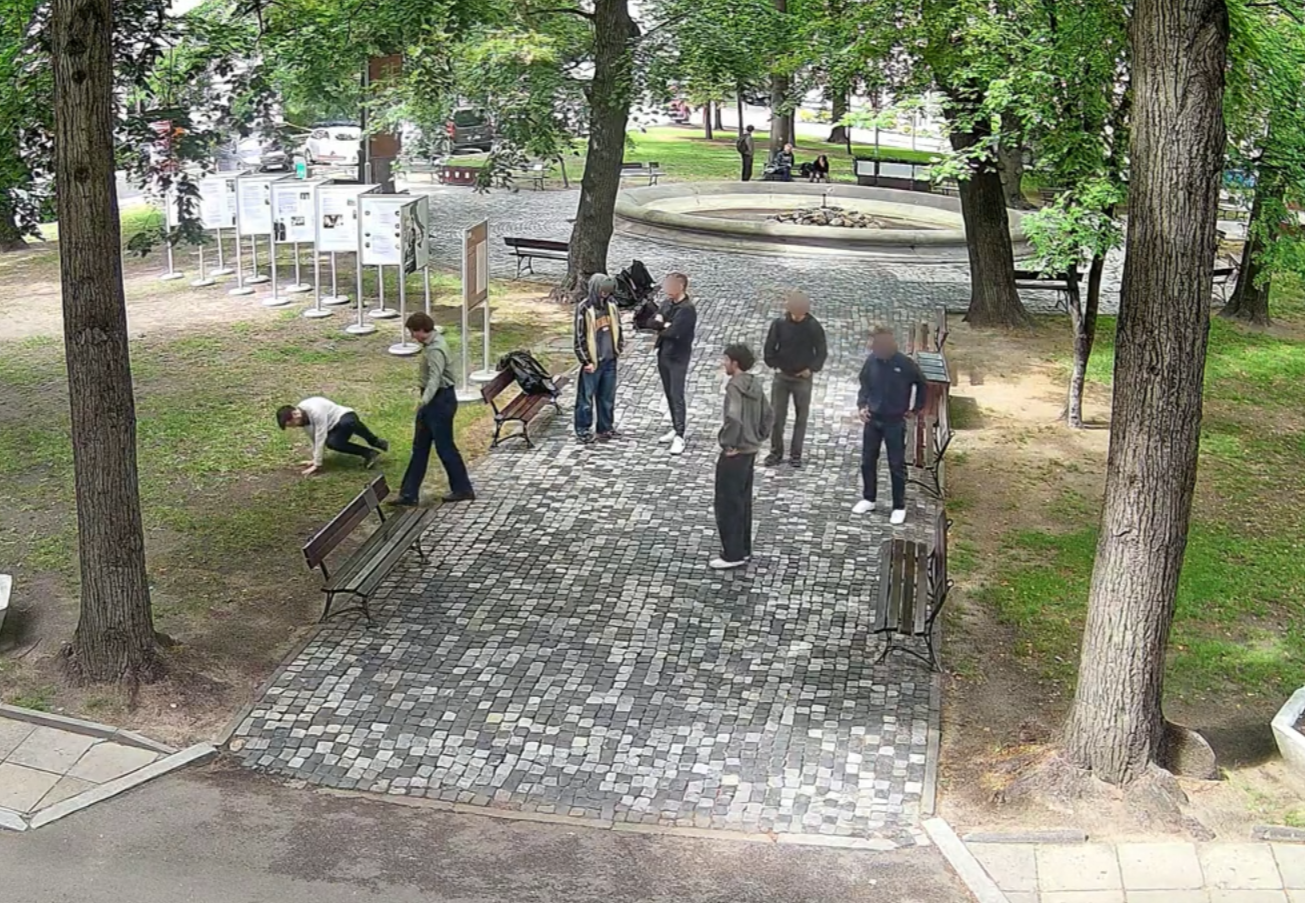
\includegraphics[width=0.95\textwidth]{images/detektor/upadek.png}
        \subcaption{Wykrycie upadku.}
    \end{subfigure}
    \hfill
    \begin{subfigure}{0.49\textwidth}
        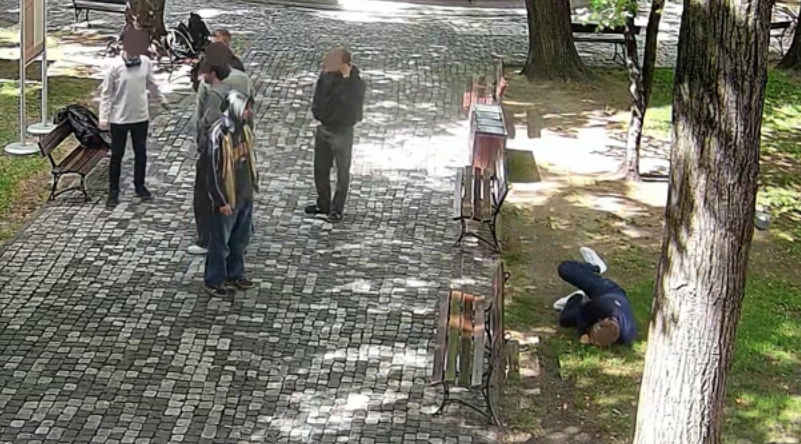
\includegraphics[width=0.95\textwidth]{images/detektor/upadek_2.png}
        \subcaption{Wykrycie upadku w innej scenie.}
    \end{subfigure}
    \caption{Przykłady poprawnej detekcji upadku człowieka.}\label{fig:detektor_upadki}
\end{figure-}

Wysoką dokładność osiągnięto również w wykrywaniu naruszeń stref zakazanych. System poprawnie rozpoznaje zarówno pełne wejścia osób w obręb wyznaczonych obszarów, jak i sytuacje graniczne, gdy postać znajduje się dopiero na samej krawędzi strefy. Świadczy to o precyzji wyznaczania punktu styku z podłożem względem zdefiniowanego wielokąta.

\begin{figure-}
    \centering
    \begin{subfigure}{0.49\textwidth}
        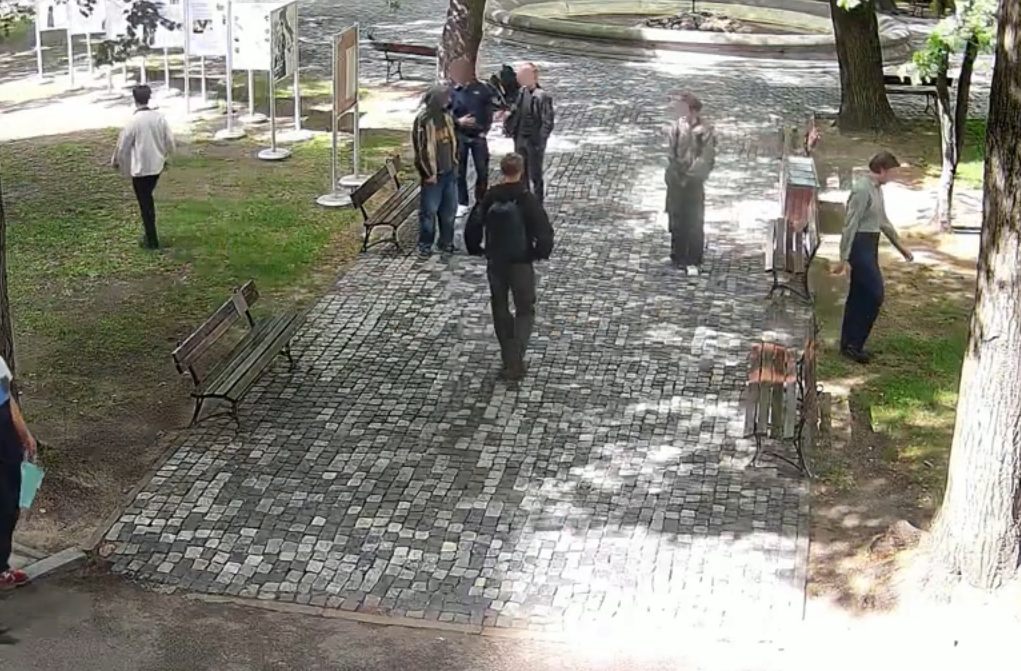
\includegraphics[width=0.95\textwidth]{images/detektor/strefa_trawnik_obie_full.png}
        \subcaption{Pełne wejście na obie strefy (lewy i prawy trawnik).}
    \end{subfigure}
    \hfill
    \begin{subfigure}{0.49\textwidth}
        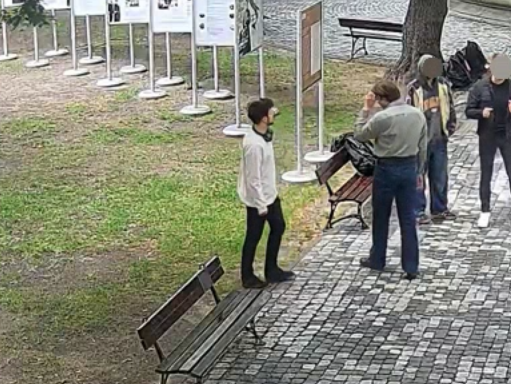
\includegraphics[width=0.95\textwidth]{images/detektor/strefa_trawnik_ledwo.png}
        \subcaption{Wejście na samą granicę strefy.}
    \end{subfigure}
    \caption{Detekcja naruszenia stref zakazanych: pełne wejście oraz sytuacja graniczna.}\label{fig:detektor_strefy}
\end{figure-}

Należy zaznaczyć ograniczenie wynikające z natury analizy opartej na ciągłości szkieletu. Przy chwilowym zasłonięciu osoby przebywającej w strefie, na przykład w wyniku przejścia za drzewem, detekcja może zostać przerwana: klasyfikator zachowań wymaga nieprzerwanego okna czasowego pozy, a wyznaczenie obecności w strefie zakłada widoczność punktu styku z podłożem. Gdy tylko postać ponownie staje się widoczna, detekcja jest wznawiana, dzięki czemu przerwy te są możliwie krótkie.

\subsection{Anonimizacja w praktyce}
Mechanizm anonimizacji skutecznie zabezpiecza dane wrażliwe. Twarze wielu osób jednocześnie, ustawionych pod różnymi kątami i z różnie zwróconymi głowami, zostają poprawnie zamazane. Jednocześnie osoba zwrócona tyłem do obiektywu, dla której model przypisuje oczom niskie prawdopodobieństwo, jest prawidłowo pomijana, co pozwala uniknąć zbędnych artefaktów.

\begin{figure-}
    \centering
    \begin{subfigure}{0.49\textwidth}
        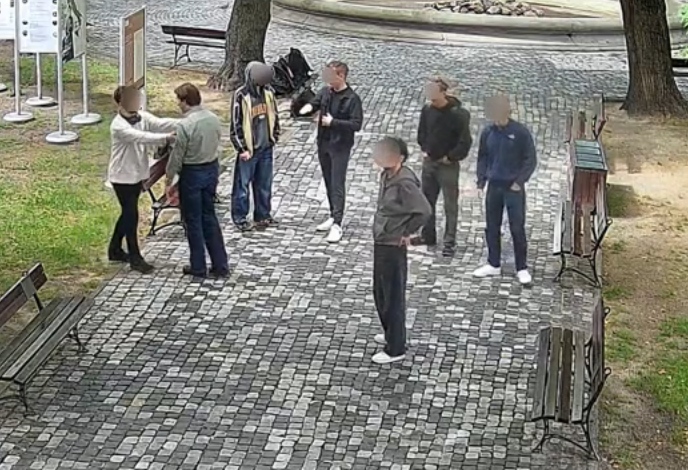
\includegraphics[width=0.95\textwidth]{images/detektor/rozmycie_twarzy.png}
        \subcaption{Rozmycie twarzy wielu osób.}
    \end{subfigure}
    \hfill
    \begin{subfigure}{0.49\textwidth}
        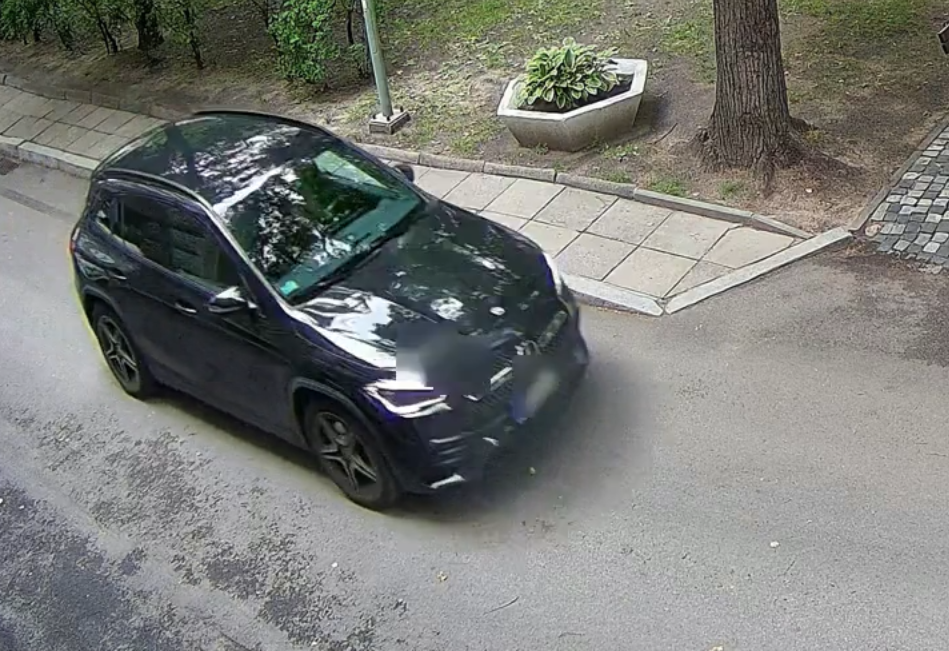
\includegraphics[width=0.95\textwidth]{images/detektor/auto.png}
        \subcaption{Rozmycie tablicy rejestracyjnej.}
    \end{subfigure}
    \caption{Działanie modułu anonimizacji: twarze przechodniów oraz tablica rejestracyjna pojazdu.}\label{fig:detektor_anonimizacja}
\end{figure-}

W przypadku tablic rejestracyjnych zdarza się, że maska rozmycia obejmuje również niewielki fragment nadwozia sąsiadujący z tablicą. Jest to nieznaczny efekt uboczny, który nie wpływa negatywnie na czytelność pozostałych cech pojazdu, a co najważniejsze, sama tablica pozostaje całkowicie nieczytelna, co jest zgodne z zamierzonym celem.

\subsection{Wpływ rozdzielczości przetwarzania}\label{subsec:detektor_imgsz}
Istotny wpływ na jakość detekcji ma stała \texttt{POSE\_IMGSZ} w module detektora, odpowiadająca parametrowi \texttt{imgsz} przekazywanemu do modeli YOLO, czyli rozmiarowi obrazu, do którego skalowana jest klatka przed inferencją. Im większa wartość tego parametru, tym dokładniejsza detekcja, szczególnie obiektów małych lub odległych od kamery (jak omawiana wcześniej klasa \texttt{knife}), lecz tym dłuższy czas przetwarzania pojedynczej klatki. Dobór tej wartości stanowi więc kompromis zależny od dostępnego sprzętu oraz od rozdzielczości obrazu wejściowego.

Przedstawione w podrozdziale~\ref{sec:detektor_wyniki} wyniki czasowe uzyskano przy wartości \texttt{POSE\_IMGSZ} równej 1600 na komputerze klasy domowej, co dało zadowalające opóźnienia przy zachowaniu wysokiej dokładności. Uruchomienie systemu na wydajniejszym sprzęcie pozwala podnieść ten parametr (a tym samym dokładność) bez pogorszenia bieżącości przetwarzania albo osiągnąć jeszcze krótsze opóźnienia przy zachowaniu dotychczasowej dokładności.
